\section{Analyse des donn\'ees}
Le but de cette manipulation est la caracterisation d'un module optique (OM) et la pr\'eparation du dispositif n\'ecessaire. Cel\`a veut dire:

\begin{center}
\fbox{
\begin{minipage}{0.75\textwidth}
Dans un premier pas se familiariser avec le dispositif:
\begin{itemize}
\item \'etudier l'efficacit\'e des PMs,
\item calibrer de l'ADC,
\item d\'eveloper la logique de l'aquisition de donn\'ees.
\end{itemize}

Ensuite, bas\'e sur les donn\'ees, calculer 
\begin{itemize}
\item le gain $G$ de l'OM,
\item la r\'esolution $\sigma_\mathrm{G}$ de l'OM,
\item le nombre moyen de photoelectrons $\langle n_{\mathrm{pe}}\rangle$ produit par trigger dans l'OM.
\end{itemize}
\end{minipage}
}
\end{center}

\ifthenelse{\boolean{showAdditional}}{
\begin{additional}
\textbf{Validation de la precedure d'adjustement:}\\
\includegraphics[width=\textwidth]{exampleAnalysis/LLFit_MC.pdf}\\
\textbf{Dispositif electrons:}\\
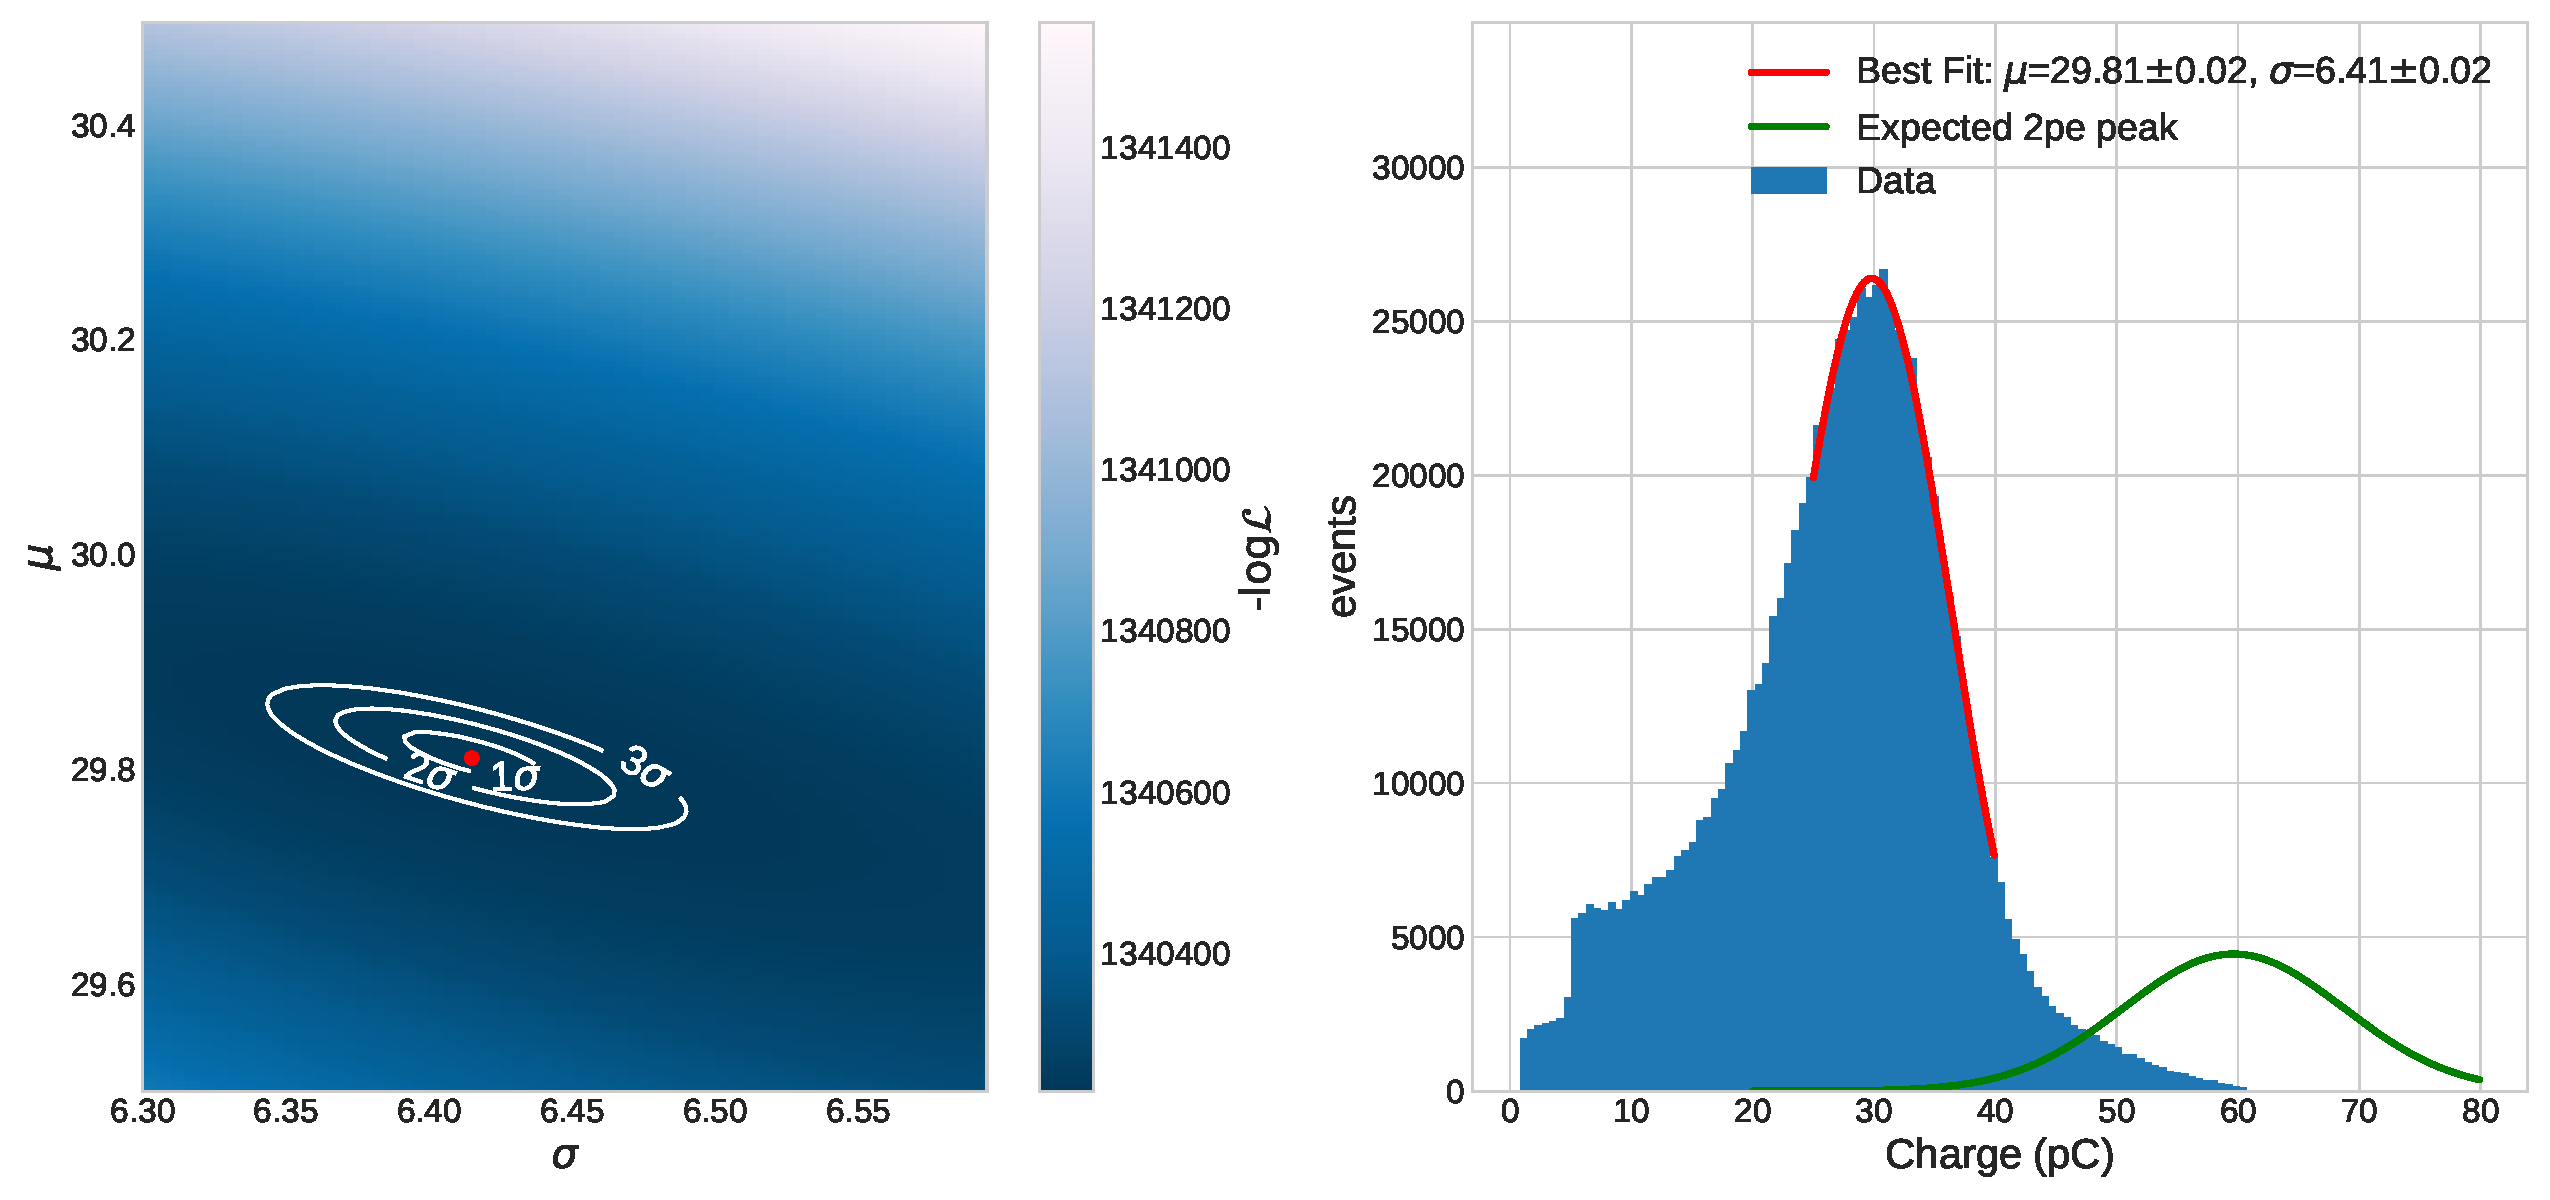
\includegraphics[width=\textwidth]{exampleAnalysis/LLFit_Data_1pe.pdf}\\
\begin{align}
G &= \mu_{\text{best}}/e = 185963 \\
\sigma_G &= \sigma_{\text{best}} / \mu_{\text{best}} = 21.52\%\\
\langle n_{\mathrm{pe}}\rangle &= \text{n.a.}
\end{align}
{\centering
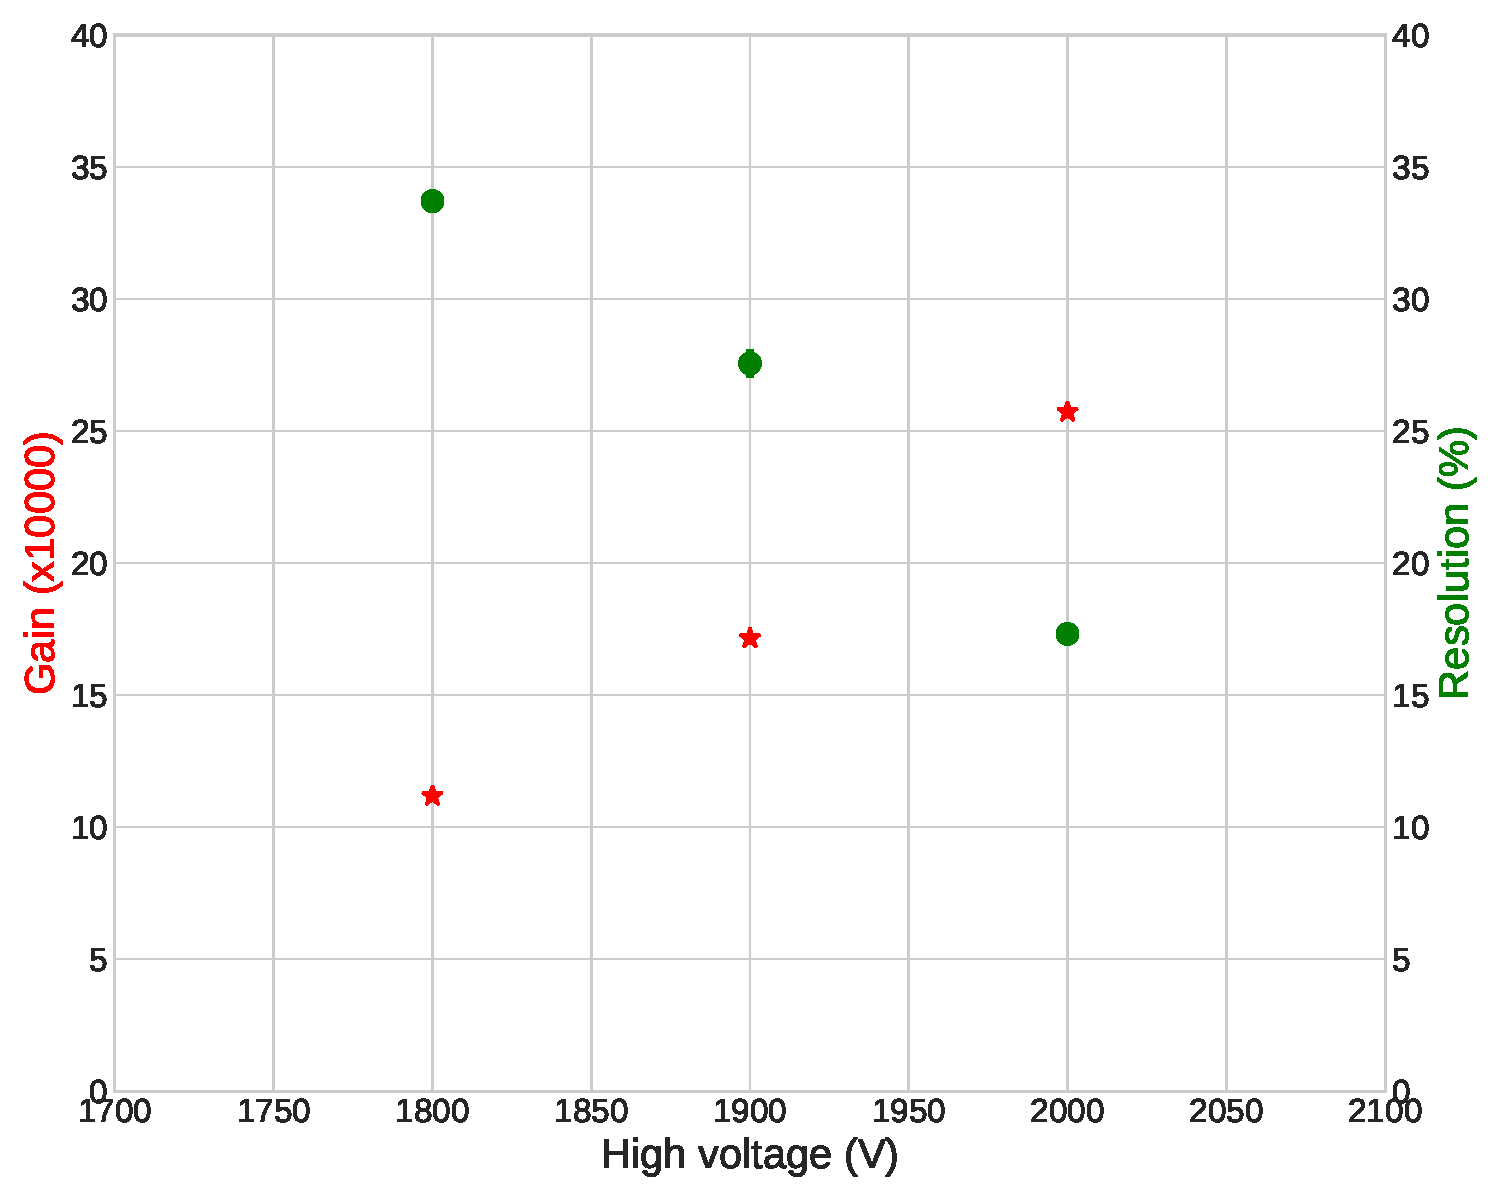
\includegraphics[width=0.7\textwidth]{exampleAnalysis/Gain_Resolution_HV.pdf}\\}
\textbf{Dispositif muons:}\\
\end{additional}
}




\pagebreak
